\documentclass[a4paper]{jpconf}
\usepackage{graphicx}
\usepackage{amsmath}
\usepackage{bm}
\begin{document}
\title{Design of a bend-twist coupled blade for a small wind turbine using multidisciplinary optimisation}

\author{Antariksh Dicholkar$^1$, Frederik Zahle$^1$, Taeseong Kim$^2$, Jessica Holierhoek$^3$ and Michael McWilliam$^1$}

\address{$^1$ DTU Wind Energy, DTU Ris{\o} campus, Frederiksborgvej 399, DK-4000 Roskilde}
\address{$^2$ DTU Wind Energy, Technical University of Denmark, Nils Koppels All{\'e}, Building 403, DK-2800 Kgs. Lyngby }
\address{$^3$ Faculty of Aerospace Engineering, TU Delft, Kluyverweg 1, 2629 HS Delft,
The Netherlands}

\ead{acdi@dtu.dk}
%%---------------------------------------------------------------------------------------------------------------------------
%%--------------------------------------------------------------------------------------------------------------------------
%\begin{abstract}
%The present study focuses on including bend-twist coupling (BTC) in the design of a 500W rotor by using a combination of parametric studies and a multidisciplinary optimisation (MDO) approach. The effectiveness of BTC is gauged through obtaining a significant decrease in the flapwise blade root bending moment accompanied by only a marginal decrease in the AEP, when compared with the baseline uncoupled turbine. Carbon outperforms glass for all fibre angles with regard to the amount of coupling seen in the blade cross-sections. Apart from flapwise bend-twist coupling, other secondary torsion couplings are also present. The steady state load response of the blade is assessed for varying positive fibre layup angles. An increase in the flapwise blade tip displacement and a reduction in the flapwise bending loads are observed. The HawtOpt2 aero-structural design tool is utilised to implement the MDO of the baseline blade.The spanwise fibre layup angle and laminate thickness distribution are the only structural design variables along with planform and operational variables to be provided with design freedom.The objective function seeks to minimise extreme flapwise bending loads and maximise the AEP through a weighted function. The performance of the optimised blades are compared for multiple combinations of the assigned weights.
%\end{abstract}
%%--------------------------------------------------------------------------------------------------------------------------
%%-------------------------------------------------------------------------------------------------------------------------
\section{Introduction}
\label{sec:intro}
Passive control of wind turbine rotors through the mechanism of material bend-twist coupling (BTC) has been sufficiently addressed in existing literature \cite{veers1998aeroelastic}. %\cite{kooijman1996bending}, \cite{karaolis1988active}. 
While early research focused on achieving power regulation by bend-twist coupling towards stall on stall-regulated constant speed rotors 
%\cite{lobitz1996enhanced}, \cite{lobitz1999load} 
, the advent of pitch regulated variable speed control strategy pivoted the research towards utilising BTC towards feather for passive load alleviation. %\cite{lobitz2003load}, \cite{lobitz2000performance}, \cite{capellaro2012design}. 
However, a large quantum of research is focused on the usage of BTC for multi-megawatt turbines with little research being conducted towards its application to small wind turbines. The present study focuses on including BTC towards feather as a mechanism for passive load alleviation, in the design of a 500W rotor by using a combination of parametric studies and a multidisciplinary optimisation (MDO) approach. The effectiveness of BTC is gauged through obtaining a significant decrease in the flapwise blade root bending moment accompanied by only a marginal decrease in the annual energy production (AEP), when compared with the baseline uncoupled turbine.

The challenge lies in developing an approach which incorporates BTC in the rotor, satisfying the multiple design constraints and presents feasible alternatives. These alternatives then have to be qualified according to their performance with only the best being carefully selected, thus resulting in a optimally performing turbine. This can be a complicated task due to the inter-dependencies of the different design requirements. The presence of complex relationships between design variables and the significant number of such variables necessitates numerical optimisation to carry out multidisciplinary design.% \cite{bottasso2012multi}, \cite{zahle2016design}.

The HawtOpt2 \cite{zahle2016design} aero-structural design tool is utilised to implement the MDO of the baseline blade and introduce BTC in the design. This study is an extension to the work conducted in the master thesis of Dicholkar \cite{dicholkar2017numerical}, wherein only the structural design variables of spanwise fibre layup angle and laminate thickness distribution were afforded design freedom with the objective function focusing on minimising extreme flapwise bending loads. In this paper along with the aforementioned structural variables, planform variables including blade length and operational variables including tip-speed ratio, are to be provided with design freedom. Additionally, the objective function seeks to minimise extreme flapwise bending loads and maximise the AEP through a weighted function. The performance of the optimised blades are to be compared for multiple combinations of the assigned weights. 


%The previous optimisation studies performed with Hawtopt2 have focused on multi-megawatt turbines, namely the DTU 10 MW reference turbine \cite{DTU10MW_1}. Zahle et. al \cite{zahle2016design} performed an aero-structural optimisation of the DTU 10MW reference rotor to maximise the annual energy production (AEP) without exceeding the design loads of the reference. Pavese et. al \cite{pavese2017design}, \cite{pavese2017aeroelastic} optimized the pre-twist distribution of swept blades designed based on the DTU 10 MW rotor. Barlas et al. \cite{barlas2016aeroelastic} conducted an aero-structural optimization of the DTU 10 MW rotor with active trailing edge flaps by assigning design freedom to the blade planform and material layup. In another study, Pavese et al. \cite{pavese2016reduced} formulated a reduced design load basis (DLB) approach that captured the effect of turbulent inflow by utilising simulated shear and extreme operating gusts, and was applied in the aero-structural optimisation of the DTU 10 MW rotor. Wandji et al. \cite{wandji2016reduction} performed an aero-structural optimisation of the DTU 10 MW rotor to minimise tower bottom fatigue loads without significant loss in AEP by utilising a weighted composite objective function.  

%This paper seeks to utilise the HawtOpt2 tool to perform an aero-structural optimisation of a 500W rotor and introduce bend-twist coupling in the process. The baseline blade being optimised for passive load alleviation is fundamentally different to that of the DTU 10 MW and operates in a different wind climate. With a much greater normalised solidity and stiffness along with smaller design loads, the limitations of the prescribed MDO workflow will inadvertently be tested.   

\section{Method}
\label{sec:method}
The baseline blade is designed using a conventional sequential design approach and has a length of 0.79 m with a uniform laminate thickness of 1 mm. Three parametric studies are conducted on the baseline blade by only varying the fibre orientations uniformly along the blade span in a discrete sense. 

First a stiffness parametric study is performed where the cross-sectional stiffnesses of the blade sections are analysed using the fully populated stiffness matrix outputs by BECAS. This analysis is performed for a carbon-fibre and a glass-fibre blade by varying the laminate fibre layup angles. The aim of this study is to primarily identify the contributions of the torsion coupling stiffness terms towards BTC, the fibre angle range that would result in twisting towards feather, the material most conducive to BTC amongst carbon and glass composites, and the dependence of the stiffnesses on cross-sectional dimensions. Next, a parametric study is performed recording the steady state load response of the carbon-fibre and glass-fibre blade at fibre angles conducive to BTC towards feather. The response of the blades is generated through aeroelastic simulation performed in the time-domain aero-servo-hydro-elastic code HAWC2. The response provides an indication of the potential benefits of implementing BTC on the 500W turbine blade. Lastly, the effect of introducing varying degrees of BTC towards feather on the fatigue response of the baseline blade is gauged. 

The baseline wind turbine blade is aero-structurally optimised using HawtOpt2 with constraints on the maximum allowable blade tip deflection, and the loads not exceeding the design loads of the reference blade. The objective function to be minimised is a compound objective comprising of extreme flapwise blade root bending moment and the AEP. The objective function is shown in Equation \ref{eq:objective_function}.
\begin{equation}
\resizebox{.9 \textwidth}{!}{ 
     $ f(\{\bm{x_p}, \bm{x_s}, \bm{x_{oper}}\},\bm{p}, w)= -\left( w \cdot \dfrac{AEP(\{\bm{x_p}, \bm{x_s}, \bm{x_{oper}}\},\bm{p})}{AEP(\{\bm{0},\bm{0},\bm{0}\},\bm{p})} + (1-w) \cdot \dfrac{M_x(\{\bm{0},\bm{0},\bm{0}\},\bm{p})}{M_x(\{\bm{x_p}, \bm{x_s}, \bm{x_{oper}}\},\bm{p})} \right)$
     }
\label{eq:objective_function}
\end{equation}
where $f$ represents the cost function, $AEP$ is the annual energy production, $M_x$ is the extreme flapwise blade root bending moment, $w$ is the weight given to the aerodynamic and structural parameters that determines the trade-off, $x_p$ are the collection of the blade planform design variables, $x_s$ is the collection of the blade structural variables, $x_{oper}$ is the collection of wind turbine control variables and $p$ represents the variables that are kept constant. $AEP(\{0,0,0\},p)$ and $M_x(\{0,0,0\},p)$ represent the AEP and the flapwise root bending moment for the baseline uncoupled rotor, respectively.

\section{Preliminary results and conclusions}
\label{sec:results}
The flapwise bending-torsion coupling with twisting towards feather is activated for positive fibre layup angles with the torsion coupling terms obtaining a negative value. Figures \ref{subfig:carbonVglass_flapvedgetors_40} and \ref{subfig:carbonVglass_otherstifftors_40} indicate the presence of secondary torsion couplings along with the primary flapwise bend-twist coupling. These secondary couplings would contribute to the final value of the induced torsion and thus either positively or negatively affect the desired outcome of BTC. Additionally, the contributions of the secondary couplings cannot be precisely quantified.      
%----------------Comparision of stiffnesses-----------
\begin{figure}[pth]
\centering
\begin{minipage}{0.35\textwidth}
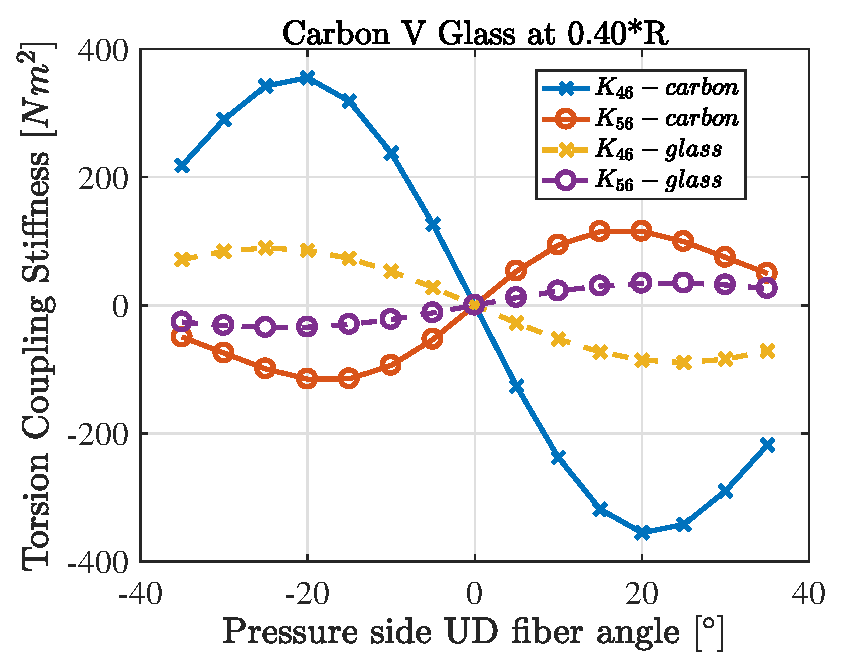
\includegraphics[width=\linewidth]{Figures/Chapter4/Stiffness/CarbonVglass_flapVedgecoupl_40_eps.eps}
\caption{\label{subfig:carbonVglass_flapvedgetors_40}Flap-torsion $K_{46}$ and edge-torsion $K_{56}$ coupling stiffness terms at 40\% blade span.}
\end{minipage}\hspace{0.10\textwidth}%
\begin{minipage}{0.35\textwidth}
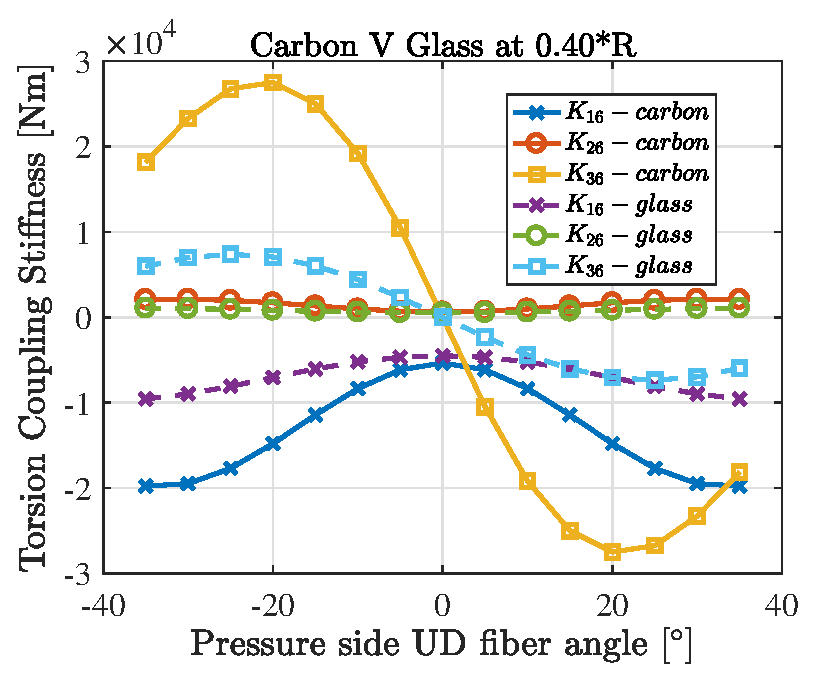
\includegraphics[width=\linewidth]{Figures/Chapter4/Stiffness/CarbonVglass_otherstiffcoupl_40_eps.eps}
\caption{\label{subfig:carbonVglass_otherstifftors_40}Edgewise shear-torsion $K_{16}$, flapwise shear-torsion $K_{26}$ and axial-torsion $K_{36}$ coupling stiffness terms at 40\% blade span.}
\end{minipage} 
\end{figure}
%----------------------------------
Figure \ref{subfig:mx_rel} shows that the maximum observed relative decrease in the flapwise blade root bending moment is 2.8\% at a fibre layup angle of 25$^\circ$ in the carbon fibre blade. The small reduction in the extreme flapwise bending load is due to the decrease in angle of attack not being significant enough for the airfoil to operate at a sub-optimal lift to drag ratio. Since only one airfoil series is used throughout the blade, this reasoning holds for the power producing mid-span and near tip region of the span. The relative change in the airfoil angle of attack near the tip is shown in Figure \ref{subfig:alphacurve_rel}.


%----------------Comparision of load response-----------
\begin{figure}[pth]
\centering
\begin{minipage}{0.35\textwidth}
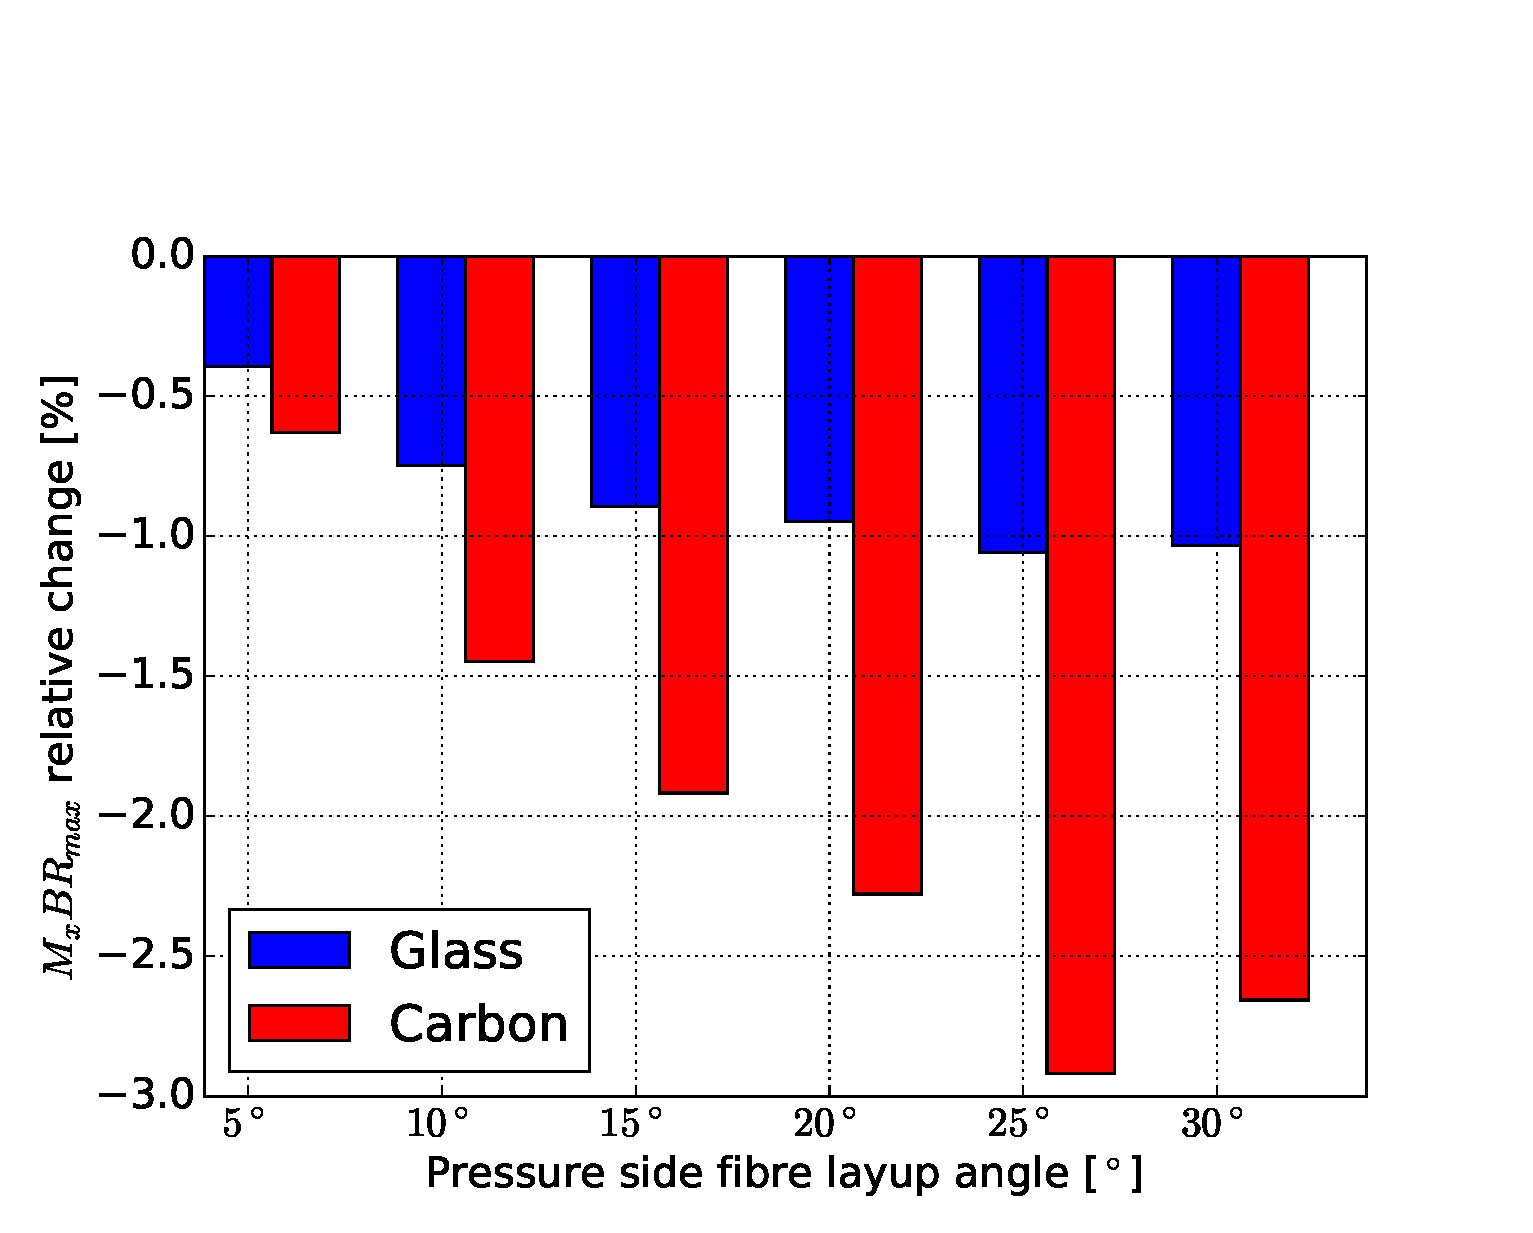
\includegraphics[width=\linewidth]{Figures/Chapter4/Load/steady_relmxbr.eps}
\caption{\label{subfig:mx_rel}Change in maximum flapwise root bending moment $M_xBR_{max}$ relative to the uncoupled blade for 10m/s rated wind speed.}
\end{minipage}\hspace{0.10\textwidth}%
\begin{minipage}{0.35\textwidth}
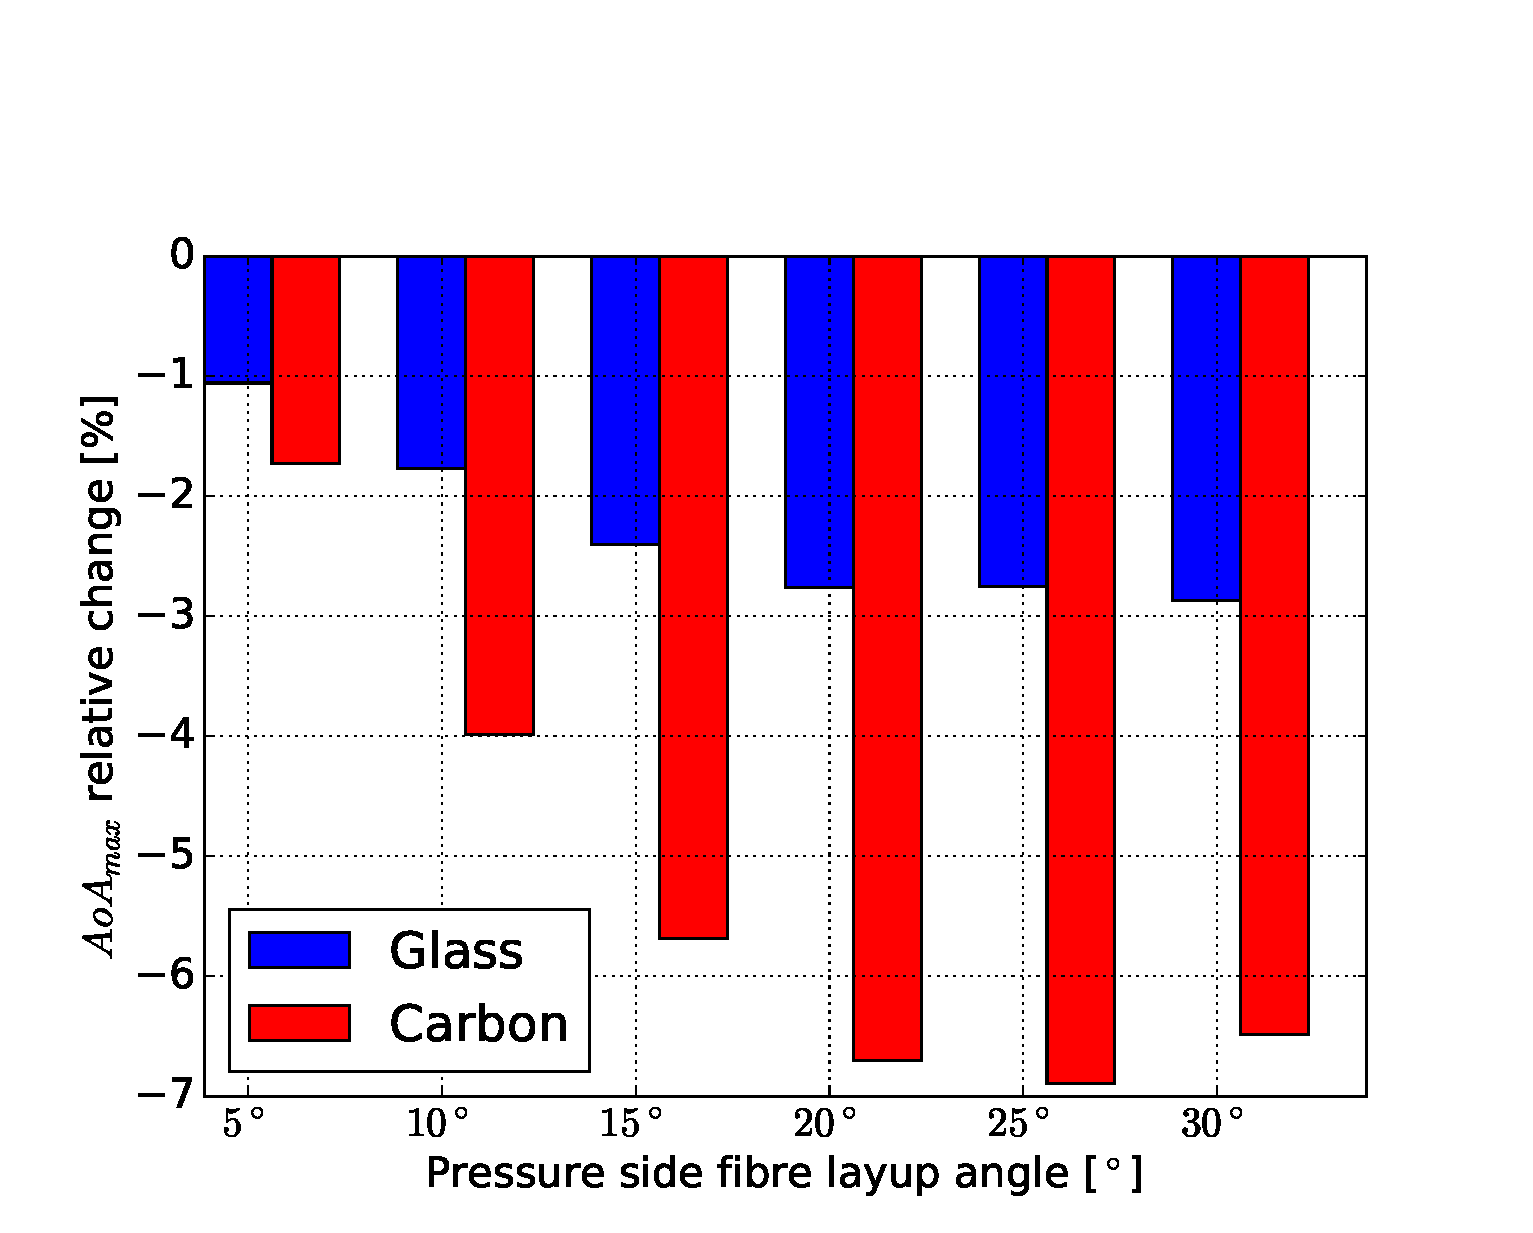
\includegraphics[width=\linewidth]{Figures/Chapter4/Load/steady_relalpha.eps}
\caption{\label{subfig:alphacurve_rel}Change in $AoA_{max}$ relative to the uncoupled case for 10m/s wind speed, at 87\% blade span.}
\end{minipage} 
\end{figure}
%----------------------------------

%\section{Preliminary conclusion}
%\label{sec:conclusion}
 Carbon outperforms glass for all fibre angles with regard to the amount of coupling seen in the blade cross-sections. Apart from flapwise bend-twist coupling, other secondary torsion couplings are also present. The small amount of reduction in the flapwise blade root bending moment points to a low degree of induced torsion as a result of the high prevalent torsional stiffness in the baseline blade, which already has a laminate thickness at the minimum manufacturing limit. A purely structural optimisation through changes in the spanwise laminate fibre layup angles may not be sufficient to produce an effective bend-twist coupled blade. A reduction in the cross-sectional stiffnesses can positively influence this outcome to a large extent. The cross-sectional stiffnesses scale with the cube of the local chord and thus altering the planform could lead to an improved response to BTC. However, this will also have an effect on the power production. Such juxtapositions in the design justify the need for an aero-structural MDO.    

%% Add the bibliography according to style iopart-num.bst
\section*{References}
\bibliographystyle{iopart-num.bst}
\bibliography{references.bib}

\end{document}


